\documentclass[apectratio=169]{beamer}
\usetheme{metropolis}           % Use metropolis theme
% For PDFs
\usepackage{pdfpages}
\usepackage{minted}
\title{Swakeup}
\subtitle{More Than A Simple Wakeup Light}
\date{\today}
\author{Elmar van Rijnswou and Maximilian Stiefel}
\institute{Uppsala University}
\begin{document}
  \maketitle

\begin{frame}{Table Of Contents}
  \setbeamertemplate{section in toc}[sections numbered]
  \tableofcontents[hideallsubsections]
\end{frame}

  \section{Introduction}
  	\begin{frame}{The Idea}
		\begin{itemize}
			\item<1-> Wakeup light which is a part of the \textit{IoT}
			\item<2-> Swakeup \ensuremath{\rightarrow} engl. "Swedish Wakeup Light"
			\item<3-> Wakes up, displays time, weather, mails, facebook
			\item<4-> Smart, small, USB charger included
		\end{itemize}
  	\end{frame}
  	\begin{frame}{System Overview}	
		\begin{figure}
			\centering
			\includegraphics[height=0.8\textheight]{../../block/block.png}
			\caption{System Overview}
		\end{figure}
	\end{frame}
  
  \section{Hardware}
  	\begin{frame}{Power Board}
		\begin{figure}
			\centering
			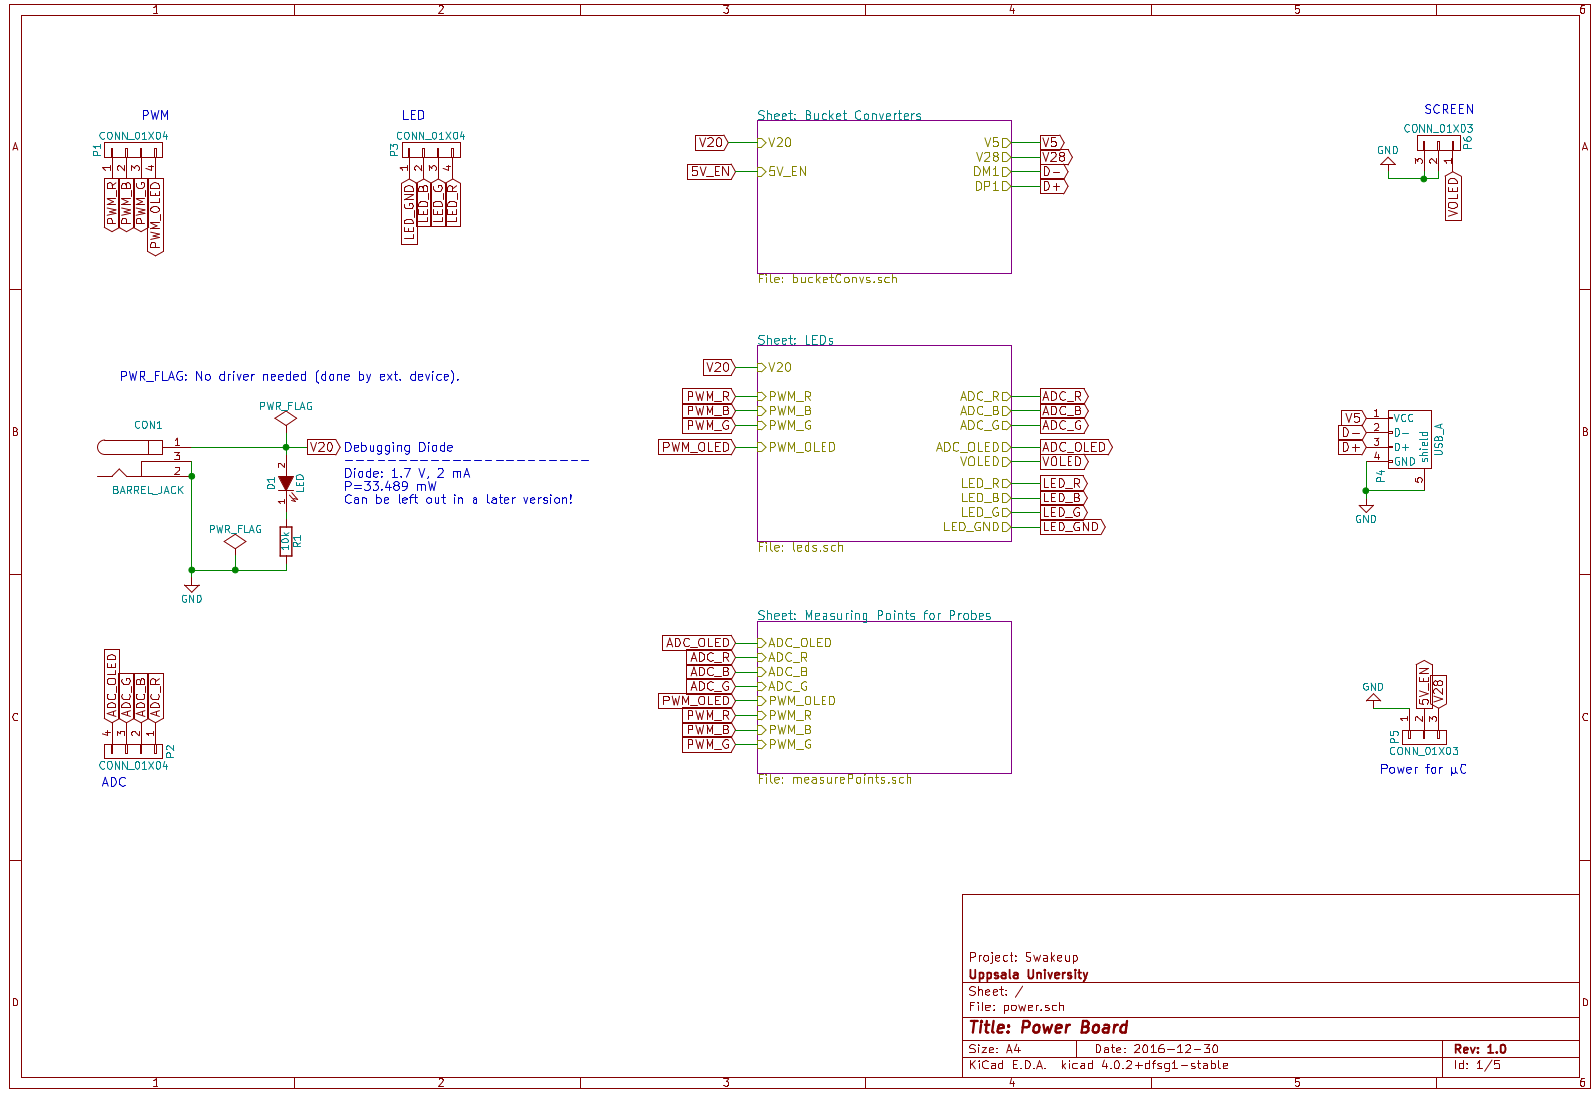
\includegraphics[width=0.95\textwidth]{./fig/power}
			\caption{Top View Of The Power Board Schematics}
		\end{figure}	
  	\end{frame}
  	\begin{frame}{Logic Board}	
		\begin{figure}
			\centering
			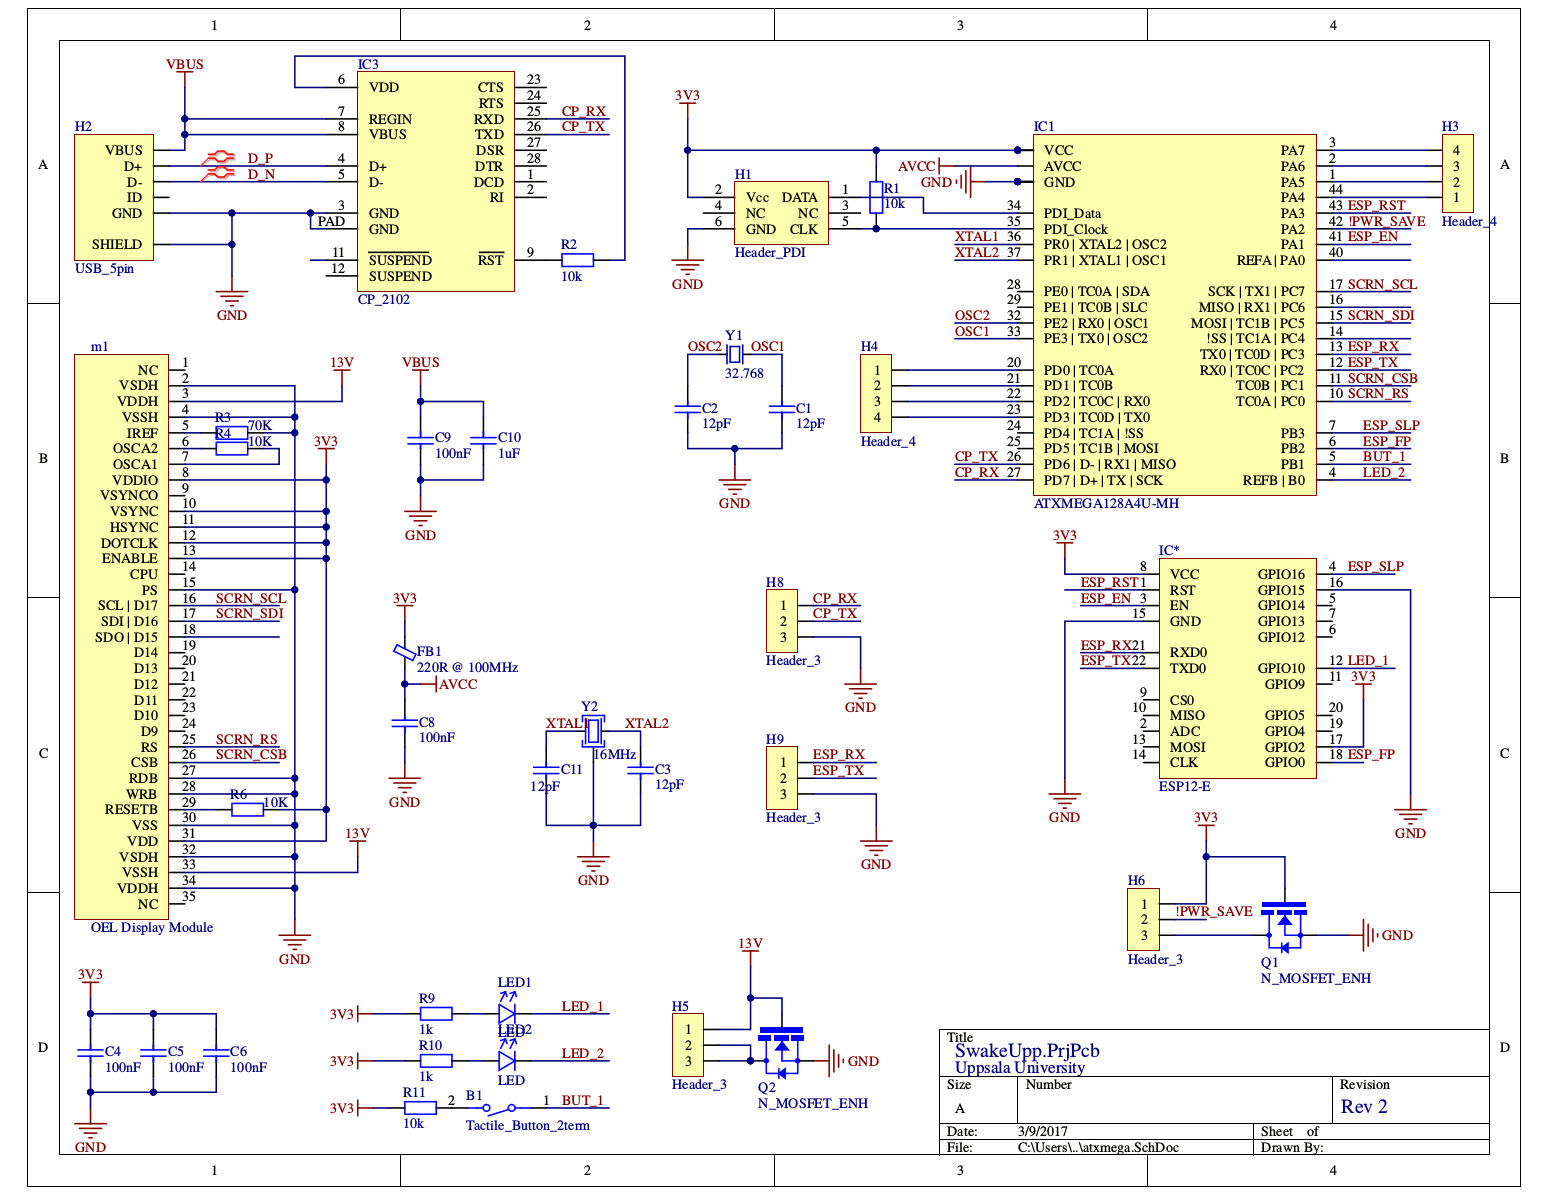
\includegraphics[height=0.8\textheight]{./fig/logic}
			\caption{Logic Board Schematics}
		\end{figure}
	\end{frame}

  \section{Software}
  	\begin{frame}{Code Structure}
		 \begin{figure}
                        \centering
                        \includegraphics[width=0.6\textwidth]{./fig/code_structure}
                        \caption{Abstract Layering Model}
                \end{figure}
  	\end{frame}
	\begin{frame}{Code Organisation}
		 \begin{figure}
                        \centering
                        \includegraphics[width=0.7\textwidth]{./fig/block_code}
                        \caption{Block Diagram Of The Code Organisation}
                \end{figure}
  	\end{frame}

\begin{frame}[fragile]{Operating System - Modules And Events}
\begin{minted}[baselinestretch=1, fontsize=\tiny, linenos,frame=single,framesep=5pt]{C}
#define MODULE_DEFINE(VAR, DESC, INIT, DEINIT, ...)     \
        Module VAR = {                                  \
                .init = INIT,                           \
                .deinit = DEINIT,                       \
                .cnt = 0,                               \
                .name = DESC,                           \
                .deps = { __VA_ARGS__ }                 \
        }
MODULE_DEFINE(CORE, "Central core", init, deinit, &TIME, &COMMAND, &ESP8266);
\end{minted}

\begin{minted}[baselinestretch=1, fontsize=\tiny, linenos,frame=single,framesep=5pt]{C}
#define EVENT_REGISTER(eventName, desc)\
        Event eventName = \
        {.eventId = __COUNTER__, .data = 0, .description = desc, .descLen = sizeof(desc) }
EVENT_REGISTER(EVENT_UART_DELIMITER, "Got UART delimiter");
\end{minted}

\begin{minted}[baselinestretch=1, fontsize=\tiny, linenos,frame=single,framesep=5pt]{C}
event_addListener(&EVENT_UART_DELIMITER, callback);
\end{minted}

\begin{minted}[baselinestretch=1, fontsize=\tiny, linenos,frame=single,framesep=5pt]{C}
event_fire(&EVENT_UART_DELIMITER, SYSTEM_ADDRESS_CAST (&delimiters[USART_ID][i]));
\end{minted}


\end{frame}	
  
	\begin{frame}{Realization (1)}
	\begin{figure}
        	\centering
                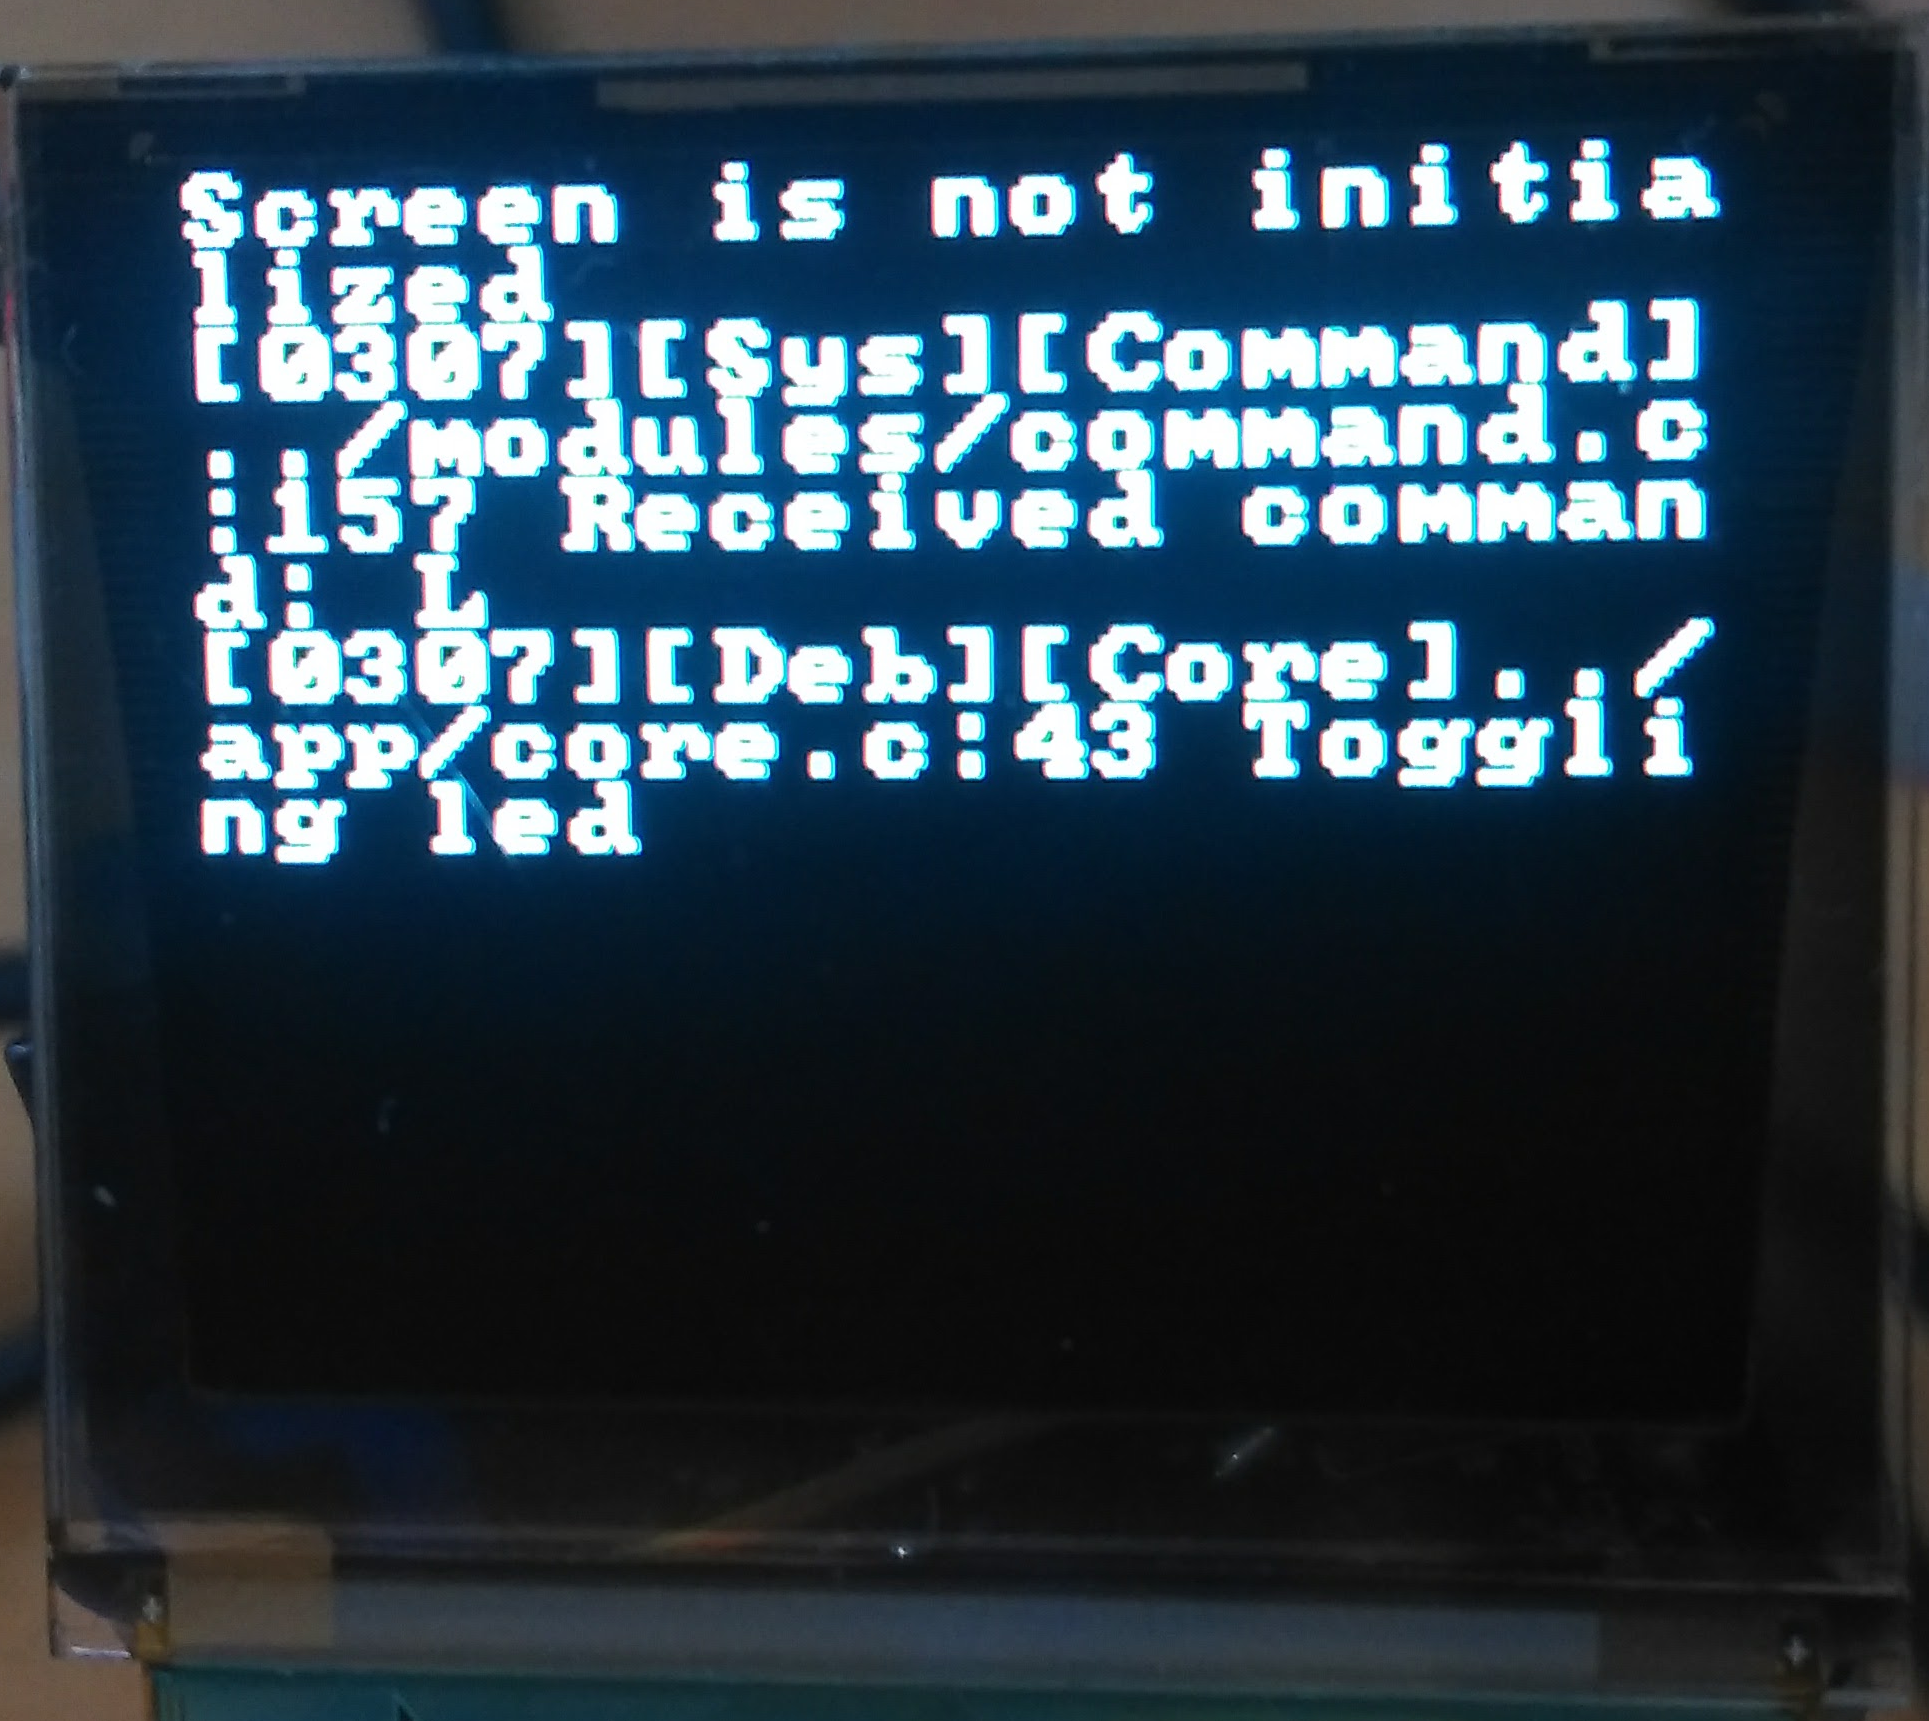
\includegraphics[width=0.6\textwidth]{./fig/screen_logger}
                \caption{Screen Logging}
        \end{figure}
	\end{frame}

	\begin{frame}{Realization (2)}
	\begin{figure}
        	\centering
                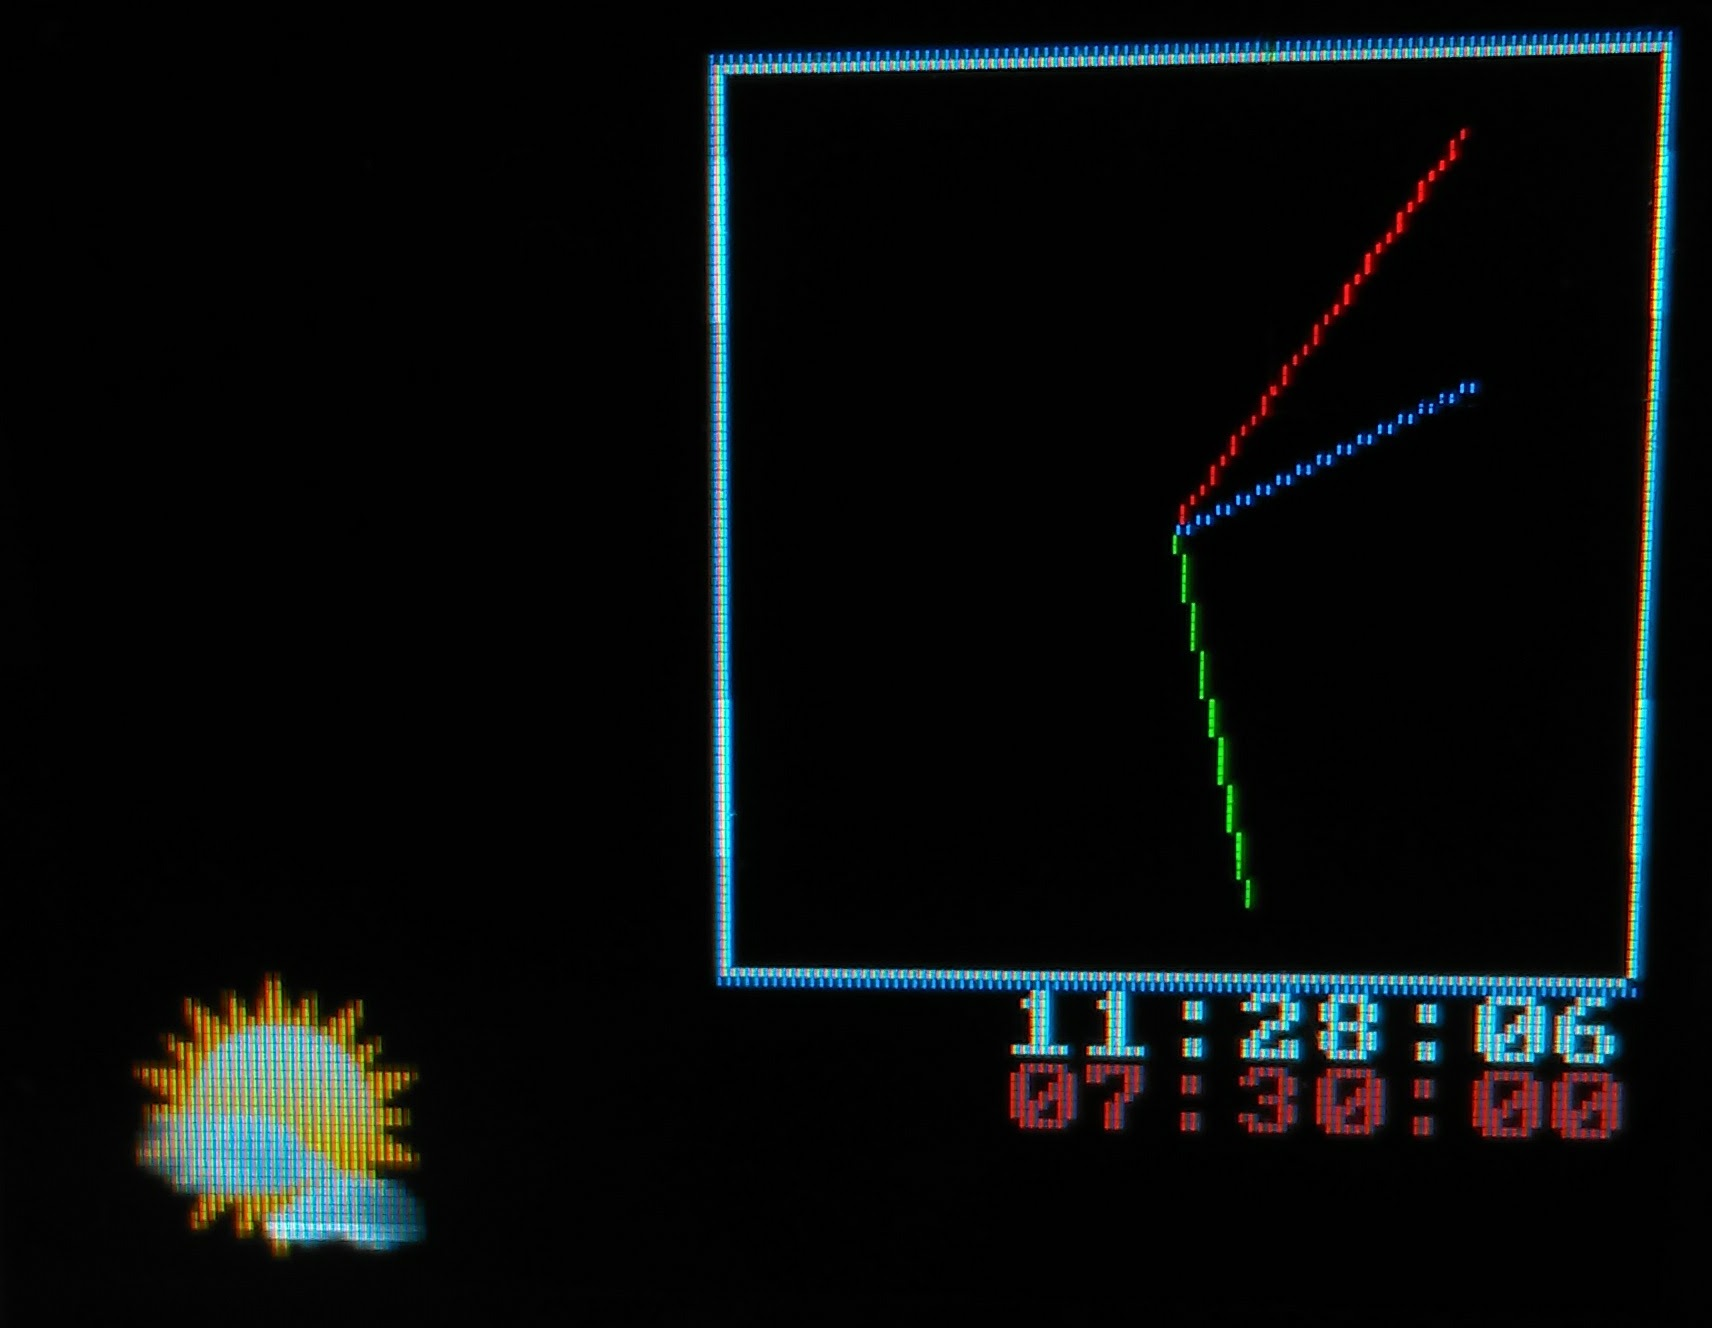
\includegraphics[width=0.6\textwidth]{./fig/clock_weather}
                \caption{Appearence Of The Clock}
        \end{figure}
	\end{frame}
	
	\begin{frame}{Realization (3)}
	\begin{figure}
        	\centering
                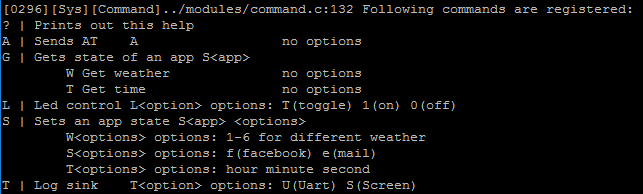
\includegraphics[width=0.6\textwidth]{./fig/command_usage}
                \caption{USART Command Interpreter}
        \end{figure}


	\end{frame}
 
  \section{Status Quo and Outlook}
  	\begin{frame}{What works? What does not? (1)}
	\footnotesize
	\begin{table}[H]
	\centering
	\begin{tabular}{lll}
	\textbf{HW Block}       & \textbf{Working}& \textbf{Problem}    \\\hline
	USB Charging    & \checkmark    &                               \\
	OLED Driver     & \checkmark    &                               \\
	Vcc for µC      & \checkmark    &                               \\
	IEEE 802.11     & \checkmark    &                               \\
	USB2UART        & \checkmark    &                               \\
	LED Driver      &               & Wrong footprint assignment    \\
	Crystal         &               & Wrong pin assignment          \\
	USB DCP         &               & Further tests necessary       \\
	\end{tabular}
	\caption{Hardware Overview: What works? What does not?}
	\label{tab:hw}
	\end{table}
  	\end{frame}

	\begin{frame}{What works? What does not? (2)}
	\tiny
	\begin{table}[H]
	\centering
	\begin{tabular}{lll}
	\textbf{SW Block}       & \textbf{Working}& \textbf{Problem}    \\\hline
	UART            & \checkmark    &                               \\
	SPI             & \checkmark    &                               \\
	EPROM           & \checkmark    &                               \\
	Timer           & \checkmark    &                               \\
	ADC             &               &                               \\
	PWM             &               &                               \\
	ESP8266         & \checkmark    &                               \\
	Terminal        & \checkmark    &                               \\
	SEP525F         & \checkmark    &                               \\
	Wifi            &               &                               \\
	Command         & \checkmark    &                               \\
	Log             & \checkmark    &                               \\
	Screen          & \checkmark    &                               \\
	Timekeeper      & \checkmark    &                               \\
	Controller      &               &                               \\
	Core            & \checkmark    &                               \\
	Weather         & \checkmark    &                               \\
	Clock           & \checkmark    &                               \\
	Social          &               &                               \\
	\end{tabular}
	\caption{Software Overview: What works? What does not?}
	\label{tab:sw}
	\end{table}

	\end{frame}
	
  	\begin{frame}{Outlook}	
		\begin{itemize}
			\item<1-> HW Rev2 has arrived
			\item<2-> LED driver will work hopefully
			\item<3-> Social connectivity and calendar functions will be implemented
		\end{itemize}
	\end{frame}

  	\begin{frame}{Contact Information}
        	\begin{center}
                \begin{table}[]
                        \begin{tabular}{ll}
                                E: & Elmar.Vanrijnswou.9818@student.uu.se \\
                                E: & Maximilian.Stiefel.8233@student.uu.se\\
                        \end{tabular}
                \end{table}
                
\includegraphics[width=0.05\textwidth]{./fig/github} \hspace{0.1cm} \url{https://github.com/s3xm3x/SwakeUp}\\
        	\end{center}
        	\begin{figure}
                	
\includegraphics[width=0.3\textwidth]{./fig/logo}
        	\end{figure}
  	\end{frame}


  \begin{frame}[standout]
	Happy Coding :) 
  \end{frame}
\end{document}
